\documentclass[11pt]{article}
\usepackage{geometry}
\usepackage{setspace}
\usepackage{amsmath}
\usepackage{graphicx}
\usepackage{hyperref}
\usepackage{graphicx}
\usepackage{amssymb}
\geometry{margin=1in}
\onehalfspacing

\title{\textbf{GPU-Accelerated Ray Tracing with CUDA:\\
A Physically Based, High-Performance Rendering System}}
\author{Luke Jachimiec}
\date{COMP 401 — Project Proposal}

\begin{document}
\maketitle

% =========================================================
\begin{abstract}
Physically based ray tracing produces highly realistic images by simulating the physical behavior of light, but its extreme computational cost has historically limited its practicality for large scenes and real-time applications. This project presents the design and implementation of a GPU-accelerated physically based ray tracing engine built from the ground up using CUDA. The system leverages massive data parallelism by mapping one ray per pixel to individual GPU threads, enabling millions of rays to be processed concurrently. Core components of the renderer include physically accurate ray-object intersection testing, material scattering models for diffuse, metallic, and dielectric surfaces, and recursive multi-bounce light transport for global illumination.

Triangle-based mesh geometry is supported through external scene loading, allowing the renderer to operate on realistic, production-scale models. Performance is evaluated through direct benchmarking of CPU single-threaded, multi-threaded, and GPU implementations across identical scenes and sampling workloads. Results demonstrate an orders-of-magnitude performance improvement when using the GPU, reducing render times from tens of minutes on the CPU to minutes on the GPU while simultaneously increasing rendering quality.

In addition to achieving significant speedup, this project provides a detailed exploration of GPU memory management, kernel design, random number generation, and optimization strategies such as bounding volume hierarchies and probabilistic path termination. The resulting system forms a modular and extensible foundation for future work in real-time ray tracing, animation, and advanced physically based rendering. This work highlights the powerful intersection of applied mathematics, computer graphics, and high-performance parallel computing in modern rendering systems.
\end{abstract}


% =========================================================
\section{Background and Introduction}

Ray tracing is a rendering technique that simulates the physical behavior of light by tracing rays from a virtual camera into a scene, computing intersections with objects, and recursively modeling the bouncing of light off surfaces.
Unlike rasterization, an older technique which approximates lighting through precomputed shaders, ray tracing naturally produces accurate shadows, reflections, refractions, and global illumination.

Despite its realism, ray tracing is extremely computationally expensive.
High-quality images often require hundreds to thousands of rays per pixel, making naive implementations take minutes or hours to render a single image at full resolution.
Through basic experimentation, rendering a 1920×1080 scene with 1000 rays per pixel can take over an hour on a CPU, which is less than ideal for almost every single scenario.

This project addresses the core challenge of ray tracing: \textbf{performance}.
By leveraging the massive parallelism of modern GPUs through CUDA, the project aims to drastically reduce render times while preserving physical accuracy.
This is directly relevant to modern real-time graphics, as current GPUs from NVIDIA and AMD now include dedicated ray tracing hardware.

While softare such as NVIDIA's OptiX and Falcor frameworks work to simplify the ray tracing process for developers, and allow easy implementation into projects, I intend to implement the ray tracer manually in CUDA to deeply explore GPU execution, memory management, performance optimization, and physically based light transport.

% =========================================================
\section{Project Description}

My goal for this project is to develop a \textbf{GPU-accelerated physically based ray tracing engine implemented in CUDA}. My vision for this project is a user will be able to input a scene consisting of meshes created on another software such as blender, and my engine would be able to ray trace their scene efficiently, and then expand to animations as well as real time ray tracing, like we see in video games



This project supports several important use cases within physically based rendering and GPU computing. First, the system is capable of rendering realistic still images using physically accurate lighting models, allowing for the visualization of soft shadows, reflections, and global illumination effects. Second, the project enables detailed visualization of reflective and refractive materials, including metals and dielectrics, which are essential for validating correct ray–material interaction behavior. Third, the framework serves as a benchmarking platform to compare the computational throughput of CPU-based and GPU-based ray tracing implementations, offering a direct study of parallel versus serial performance. Finally, the system allows exploration of the feasibility of real-time or near-real-time ray tracing by measuring rendering performance under progressively increasing workloads and scene complexity.


At a high level, the system follows a structured pipeline beginning with scene setup, during which the camera model, geometric objects, and material parameters are defined on the host. Once initialized, scene data is transferred to GPU global memory, where it remains resident for the duration of the rendering process. Parallel ray generation is then executed using CUDA kernels, with each GPU thread responsible for computing the color of a unique pixel. These rays undergo ray–object intersection testing against the scene geometry, followed by material shading and recursive ray scattering as determined by surface properties.  Finally, the computed image is transferred back to the host and written to disk as a PNG file for analysis and visualization.

\subsection*{Experimental Plans}

A structured set of experiments will be conducted to evaluate both the mathematical and computational performance of the system. Rays-per-second throughput will be measured for both CPU and GPU implementations to quantify the speedup achieved through parallel execution. Total render times for identical scenes will be compared across platforms to evaluate scalability. Additionally, the performance impact of different material types will be measured to determine how diffuse, reflective, and refractive surfaces influence computational workload. Together, these experiments establish a rigorous framework for validating both the numerical integrity and performance efficiency of the ray tracing system.


% =========================================================
\section{Foundations}

This project is grounded in several foundational areas of computer science:

\begin{itemize}
    \item{Parallelism}
    \item{ray-object intersections within a scene}
    \item{materials}
    \item{Optimization techniques}
    \item{CUDA}
    \item{CPU vs GPU performance benchmarking}
\end{itemize}

\subsection{CUDA and GPU parallelism}

Modern physically based rendering relies heavily on massive parallel computation in order to simulate light efficiently. With an NVIDIA GPU, I am able to gain access to NVIDIA's \textit{Compute Unified Device Architecture} (CUDA) framework to execute ray tracing algorithms on the \textit{Graphics Processing Unit} (GPU) in order to utilize the maximum power needed to run a ray tracing algorithm efficiently and accurately.

Traditional \textit{Central Processing Units} (CPUs) are optimzized for low latency execution of a small number of complex instructions. They feature sophisticated control flow, large caches, and a small number of cores optimized for sequential performance.

In contrast, GPUs are designed for throughput oriented workloads consisting of millions of independent, lightweight computations. Ray tracing is a very good reason to use GPU Acceleration because each ray can be evaluated largely independently from eachother. This maps naturaly to the GPU's architecture, where thousands of threads can be launched simultaneously, each calculating ray intersections, shading, and light transport for each ray all at the same time as every other ray. 

Through the process of creating this project, I will dive deeper into the GPU architecture to gain a better understanding on how to properly parallel program using the GPU, and all of the intricate details involved with GPU parallel programming. 

\subsection{Ray-Object Intersections Within a Scene}

At the core of any ray tracing system lies the problem of determining how rays interact with the objects in a three-dimensional scene. The ray-object intersection computation forms the geometric foundation upon which all lighting, shading, and visibility calculations are built. Given a ray emitted into the scene, the ray tracer must determine if, where, and with which object the ray first intersects. This section presents the mathematical structure of rays, the formulation of intersection tests for basic geometric primitives, and the computational role these tests play in the rendering equation framework.

\subsubsection{Mathematical Representation of a Ray}

A ray in three-dimensional Euclidean space is defined parametrically as
\begin{equation}
\mathbf{r}(t) = \mathbf{o} + t\mathbf{d}, \quad t \geq 0,
\end{equation}
where $\mathbf{o} \in \mathbb{R}^3$ is the ray origin, $\mathbf{d} \in \mathbb{R}^3$ is a normalized direction vector, and $t$ is a scalar parameter measuring distance along the ray. The ray represents all points extending forward from the origin in the specified direction.

In ray tracing, rays are generated for primary visibility (camera rays), shadow testing, and recursive transport of reflected and transmitted light. Each ray is evaluated independently to determine its interaction with scene geometry.

\subsubsection{The Ray-Surface Intersection Problem}

Given a geometric surface $S \subset \mathbb{R}^3$, the ray-object intersection problem consists of solving
\begin{equation}
\mathbf{o} + t\mathbf{d} \in S
\end{equation}
for the smallest positive $t$. This value corresponds to the first visible surface encountered along the ray's path. If no solution exists for $t \geq 0$, the ray escapes the scene and typically contributes background illumination.

\subsubsection{Sphere Intersection}

The simplest nontrivial intersection test is for a sphere of radius $R$ centered at $\mathbf{c}$. A point $\mathbf{x}$ lies on the sphere if
\begin{equation}
\|\mathbf{x} - \mathbf{c}\|^2 = R^2.
\end{equation}
Substituting the ray equation $\mathbf{r}(t)$ yields
\begin{equation}
\|\mathbf{o} + t\mathbf{d} - \mathbf{c}\|^2 = R^2,
\end{equation}
which expands into a quadratic equation in $t$,
\begin{equation}
at^2 + bt + c = 0,
\end{equation}
with coefficients
\begin{align}
a &= \mathbf{d} \cdot \mathbf{d}, \\
b &= 2(\mathbf{o} - \mathbf{c}) \cdot \mathbf{d}, \\
c &= \|\mathbf{o} - \mathbf{c}\|^2 - R^2.
\end{align}
Real solutions exist only if the discriminant $b^2 - 4ac \geq 0$. The smallest positive root corresponds to the visible intersection. This computation provides the hit location, surface normal, and distance required for shading calculations.

\subsubsection{Triangle and Mesh Intersections}

In most realistic scenes, objects are composed of triangle meshes rather than analytic primitives. A triangle defined by vertices $\mathbf{v}_0, \mathbf{v}_1, \mathbf{v}_2$ can be intersected using barycentric coordinates. The intersection point satisfies
\begin{equation}
\mathbf{o} + t\mathbf{d} = \mathbf{v}_0 + u(\mathbf{v}_1 - \mathbf{v}_0) + v(\mathbf{v}_2 - \mathbf{v}_0),
\end{equation}
with constraints
\begin{equation}
u \geq 0, \quad v \geq 0, \quad u + v \leq 1.
\end{equation}
Solving for $(t, u, v)$ determines both the intersection position and whether the ray passes through the triangle interior. This formulation generalizes intersection testing to any polygonal surface represented as a mesh.

\subsubsection{Surface Normals and Shading Geometry}

Once an intersection is found, the surface normal vector $\mathbf{n}$ is required to evaluate illumination. For analytic primitives such as spheres, the normal is computed as
\begin{equation}
\mathbf{n} = \frac{\mathbf{x} - \mathbf{c}}{\|\mathbf{x} - \mathbf{c}\|}.
\end{equation}
For triangle meshes, the normal may be constant over each triangle (flat shading) or interpolated from per-vertex normals using barycentric weights (smooth shading).

The surface normal defines the local coordinate system used to evaluate the rendering equation and determines how incoming and outgoing light directions are measured relative to the surface.


\subsubsection{Computational Challenges}

Ray-object intersection testing dominates the computational cost of ray tracing. In scenes containing millions of triangles, naively testing every ray against every object results in extremely complex and cost inefficient algorithms. This motivates the use of acceleration structures such as bounding volume hierarchies (BVHs) and spatial partitioning methods, which dramatically reduce the number of intersection tests required per ray. This idea will be researched and implemented later.

\subsubsection{}

Each of these equations can be trivially translated to code to be used by our algorithm at any given time. These equations are  the geometric backbone for all light transport simulations used in this project. Without a way to mathematically model each of these intersections, this ray tracing, along with countless other applications would not be possible, as there would be no way for the computer to know if objects are being hit with a ray.  



\subsection{Material Models and Scattering Implementation}

In a ray tracing system, materials determine how rays behave after intersecting a surface. Rather than computing illumination directly from closed-form lighting models, this project uses a \textbf{scattering-based approach}, where each material probabilistically generates a new ray based on surface properties. Each material defines a \texttt{scatter()} function that controls how rays reflect, refract, or diffuse after impact.

All materials inherit from a common abstract interface:
\begin{itemize}
    \item Input: incoming ray, surface hit record
    \item Output: scattered ray, attenuation (color scaling factor)
\end{itemize}

This allows polymorphic material behavior while maintaining a uniform ray traversal pipeline.

\begin{figure}[h]
    \centering
    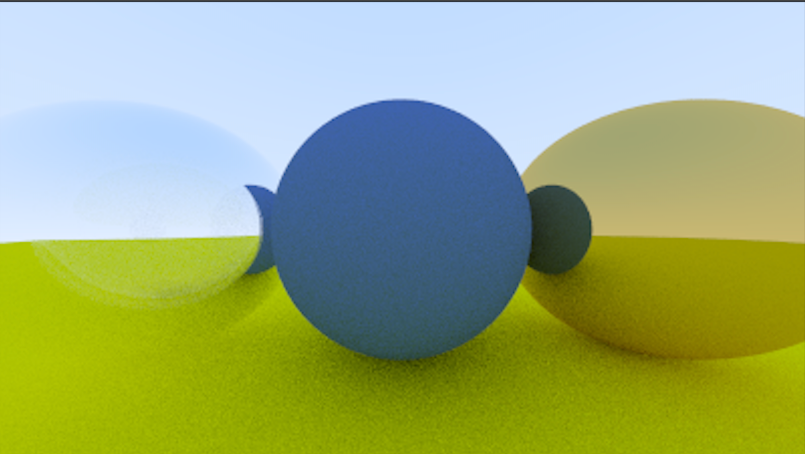
\includegraphics[scale = 0.35]{lambertianBall.png}
    \caption{From left, Dielectric, Lambertian, and Metallic material}
\end{figure}

\subsubsection{Lambertian (Diffuse) Material Implementation}

Lambertian materials simulate rough, matte surfaces that scatter light uniformly in all directions. In implementation, this is achieved by randomly sampling a direction inside a unit hemisphere oriented around the surface normal.

\subsubsection{Data Representation}

Each Lambertian material stores:
\begin{itemize}
    \item An RGB albedo vector $\mathbf{a} = (a_r, a_g, a_b)$
\end{itemize}

\subsubsection{Scattering Algorithm for Lambertian Materials}

Given a hit point $\mathbf{p}$ and surface normal $\mathbf{n}$:
\begin{enumerate}
    \item Generate a random unit vector $\mathbf{r}$ inside the unit sphere.
    \item Compute scattered direction:
    \[
    \mathbf{d}_{out} = \mathbf{n} + \mathbf{r}
    \]
    \item Construct the scattered ray:
    \[
    \mathbf{R}_{out}(t) = \mathbf{p} + t\mathbf{d}_{out}
    \]
    \item Set attenuation to the material albedo.
\end{enumerate}

This approach avoids expensive trigonometric sampling and produces visually correct diffuse scattering with minimal computational overhead.

\subsubsection{Metallic (Reflective) Material Implementation}

Metallic materials reflect rays about the surface normal, simulating mirror-like behavior. Unlike Lambertian materials, the output ray direction is deterministic with optional random perturbation for surface roughness.

\subsubsection{Data Representation}

Each metallic material stores:
\begin{itemize}
    \item Albedo vector $\mathbf{a}$
    \item Roughness parameter $f \in [0,1]$
\end{itemize}

\subsubsection{Scattering Algorithm for Metallic Materials}

Given incoming direction $\mathbf{d}$ and normal $\mathbf{n}$:
\begin{enumerate}
    \item Compute perfect reflection:
    \[
    \mathbf{r} = \mathbf{d} - 2(\mathbf{d} \cdot \mathbf{n})\mathbf{n}
    \]
    \item Apply surface roughness:
    \[
    \mathbf{r}' = \mathbf{r} + f \cdot \text{random\_unit\_vector()}
    \]
    \item Construct scattered ray.
    \item Reject rays that point below the surface (dot product check).
\end{enumerate}

Higher roughness values blur reflections by randomly perturbing the outgoing direction.

\subsubsection{Dielectric (Refractive) Material Implementation}

Dielectric materials simulate transparent objects such as glass and water. These require handling both reflection and refraction depending on the angle of incidence.

\subsubsection{Data Representation}

Each dielectric material stores:
\begin{itemize}
    \item Index of refraction $\eta$
\end{itemize}

\subsubsection{Scattering Algorithm for Dielectric Materials}

Given incoming ray direction $\mathbf{d}$ and normal $\mathbf{n}$:
\begin{enumerate}
    \item Compute refraction ratio based on whether the ray is entering or exiting.
    \item Attempt refraction using Snell's law.
    \item Compute reflection probability using Schlick's approximation.
    \item Use a random float to probabilistically choose between:
    \begin{itemize}
        \item Specular reflection
        \item Refraction
    \end{itemize}
    \item Construct scattered ray accordingly.
\end{enumerate}

This probabilistic branching produces realistic glass behavior including total internal reflection.

\subsubsection{Material Polymorphism and Ray Dispatch}

All material types inherit from a common \texttt{material} interface:
\begin{verbatim}
bool scatter(const ray& r_in, 
             const hit_record& rec,
             vec3& attenuation,
             ray& scattered);
\end{verbatim}

\textbf{At runtime:}

The ray intersects a geometric object within the scene, the object's material pointer is accessed, and the appropriate \texttt{scatter()} function executes.

This design enables dynamic material type switching, a clean separation of geometry and shading logic, and extensibility for additional materials.

\subsubsection{Recursion}

Each scattered ray recursively triggers another ray trace. To prevent infinite recursion, a maximum recursion depth is enforced. If rays do not find a valid scattering surface, or are sent off into the sky, they are terminated early as well, and their properties are calculated accordingly.

This guarantees numerical stability and bounded execution time per pixel. As well as proper ray tracing of the sky or other void like instances within the scene, so a ray does not travel infinetly in a certain direction without hitting anything relevant.






\subsection{Optimization}

With a computationally complex algorithm, it is extremely important to refer to some optimization techniques instead of strictly calculating every single ray throughout the scene. 

For instance, an image of 1920x1080 pixels could utilize 1,000 rays per pixel, each with a maximum depth of 50. Before any of those rays hit a single object within the scene, there are already 2,073,600,000 rays initially being sent into the scene, and once they begin intersecting and bouncing 50 times each, the number of rays increases to 103,680,000,000 throughout the entire process. 

There is then the question of how many calculations a CPU must make to calculate just one ray. To calculate this, we will take CPU \textit{floating-point operations} (FLOPs), assuming triangle geometry, BVH acceleration, and standard materials.

\begin{itemize}
    \item 800 to 2400 FLOPs for BVH traversal (before any object is hit)
    \item 70 FLOPs for ray-triangle intersection
    \item 50 - 100 FLOPs for Hit record Construction
    \item For different materials scattering cost
    \begin{itemize}
        \item Lambertian: 40-70 FLOPs
        \item Metallic: 50-80 FLOPs
        \item Dielectric: 90-140 FLOPs
    \end{itemize}
    \item 40 FLOPs Random Number Generation 
    \item 30-50 FLOPs during ray construction for next bounce
\end{itemize}

All of this for a single ray bounce amounts to, on average, 1100 to 2700 FLOPs

Now with a max depth of 50, this number increases to 55,000 to 135,000 per single ray. So if each ray is performing on average 100,000 floating point operations each bounce, and over the entire scene and every ray and ray bounce \[(10^{11} \text{ rays}) \times (10^{5} \text{ FLOPs per ray}) = 10^{16} \text{ total FLOPs} \] which comes out to around 10,368,000,000,000,000 (10 quadrillion) non-trivial operations over the course of the entire scene. So we can easily see why it is important to approximate and optimize some of these calculations to allow the algorithm to run more efficiently. OVer the course of this project, I will dive into different optimization techniques to better understand the shortcuts taken in order to provide an efficient algorithm able to produce high quality images quickly, and especially in gaming, rendering a single frame in 16.67 milliseconds to achieve the coveted 60 FPS in gaming

\subsection{CUDA Development}

This project uses the CUDA programming model to implement massively parallel ray tracing on the GPU. CUDA uses a C/C++ based interface that allows programmers to offload compute-intensive kernels to the GPU while coordinating execution from the CPU (host). This section outlines the fundamental structure of CUDA programs, the execution model, memory organization, and how ray tracing algorithms are mapped to GPU kernels.

\subsubsection{Structure of a Basic CUDA Program}

A CUDA program is divided into two components. It's \textit{Host code} executes on the CPU and orchestrates memory allocation, kernel launches, and data transfer. The \textit{Device code} executes on the GPU and contains the parallel kernel functions. A minimal CUDA program should consist of 

\begin{enumerate}
    \item Allocation of device memory using \texttt{cudaMalloc}
    \item Transfer of input data using \texttt{cudaMemcpy}
    \item Kernel launch using the \texttt{<<<grid, block>>>} syntax
    \item Transfer of results back to the host
    \item Deallocation of device memory
\end{enumerate}

\subsubsection{Thread, Block, and Grid Execution Model}

When a CUDA kernel is launched, thousands of threads are created simultaneously. These threads are organized as:
\begin{itemize}
    \item \textbf{Threads}: Individual execution units
    \item \textbf{Blocks}: Groups of threads that can synchronize and share fast shared memory
    \item \textbf{Grids}: Collections of blocks launched by a kernel
\end{itemize}

\begin{figure}[h]
    \centering
    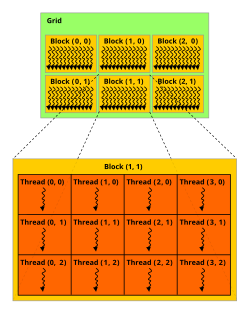
\includegraphics[width=0.5\linewidth]{Block-thread.png}
    \caption{Diagram of GPU Architecture}
\end{figure}

Each thread computes a unique index using built-in variables such as:
\begin{verbatim}
int idx = blockIdx.x * blockDim.x + threadIdx.x;
\end{verbatim}

This indexing scheme allows data-parallel algorithms to assign one thread per element, pixel, or ray.

\subsubsection{Basic CUDA Kernel Example}

The following example demonstrates a simple vector addition kernel:

\begin{verbatim}
__global__ void vecAdd(float* a, float* b, float* c, int n) {
    int idx = blockIdx.x * blockDim.x + threadIdx.x;
    if (idx < n) {
        c[idx] = a[idx] + b[idx];
    }
}
\end{verbatim}

The host launches the kernel as follows:

\begin{verbatim}
int threadsPerBlock = 256;
int blocks = (n + threadsPerBlock - 1) / threadsPerBlock;
vecAdd<<<blocks, threadsPerBlock>>>(d_a, d_b, d_c, n);
\end{verbatim}

This illustrates the fundamental GPU execution pattern used throughout CUDA-based ray tracing.

\subsubsection{CUDA Memory Model}

CUDA exposes several layers of memory with different performance characteristics. Global memory is large and accessible by all threads but has high access latency. Shared memory is significantly faster and is shared among threads within the same block, making it useful for caching frequently accessed data. Registers provide the fastest memory access and are private to each individual thread. 

In GPU-based ray tracing, global memory is primarily used to store persistent scene data such as geometry, material parameters, ray buffers, and the output framebuffer. Because rays traverse the scene using largely random memory access patterns, memory bandwidth and cache behavior heavily influence overall performance. Efficient memory layout and access patterns are therefore critical to achieving high ray throughput.


\subsubsection{Mapping Ray Tracing to CUDA Kernels}

In this project, ray tracing is parallelized using \textbf{one GPU thread per pixel}. Each thread:
\begin{enumerate}
    \item Generates a primary ray from the camera
    \item Traces the ray through the scene
    \item Computes surface intersections
    \item Applies material scattering
    \item Accumulates color contributions
    \item Writes the final color to the output buffer
\end{enumerate}

This parallelism approach allows millions of rays to be processed simultaneously, without having to wait on the other rays to be processed before continuing to the next ray.



\subsubsection{Random Number Generation in CUDA}

Ray Tracing requires per-thread random number generation. Each thread maintains an independent RNG state to ensure statistical independence across rays. Lightweight generators such as linear congruential generators (LCGs) or XORSHIFT are preferred over heavyweight library calls to reduce overhead.

Overall, CUDA random number generation is relatively more efficient compared to a random number generator you'd see on a CPU, and allows each ray to have their own psuedo random algorithm, which helps maintain randomness throughout the rendering, to achieve the most random possible outcome for each ray, which helps with image quality.


\subsubsection{Importance of CUDA}

The majority of this project will be using CUDA's architecture in order to achieve an efficient ray tracing algorithm. The purpose of this entire project was to give myself insight into a completely different type of parallel computing, and get my fingers dirty with high performance computing. Ray tracing is simply the implementation of these parallel computing ideas, as it is a very common practice to use GPU parallelism to efficiently ray trace. 



\subsection{CPU vs GPU performance benchmarking}
In my preliminary testing of a basic Ray Tracing program, I was able to test and achieve many different results, including single threaded CPU performance, multi-threaded CPU performance, and GPU performance

For all of these tests, I created and rendered the same scene, consisting of 3 big balls, each with one of the three main materials, surrounded by a random assortment of smaller spheres, following similar material and color properties.



\begin{figure}[h]
    \centering
    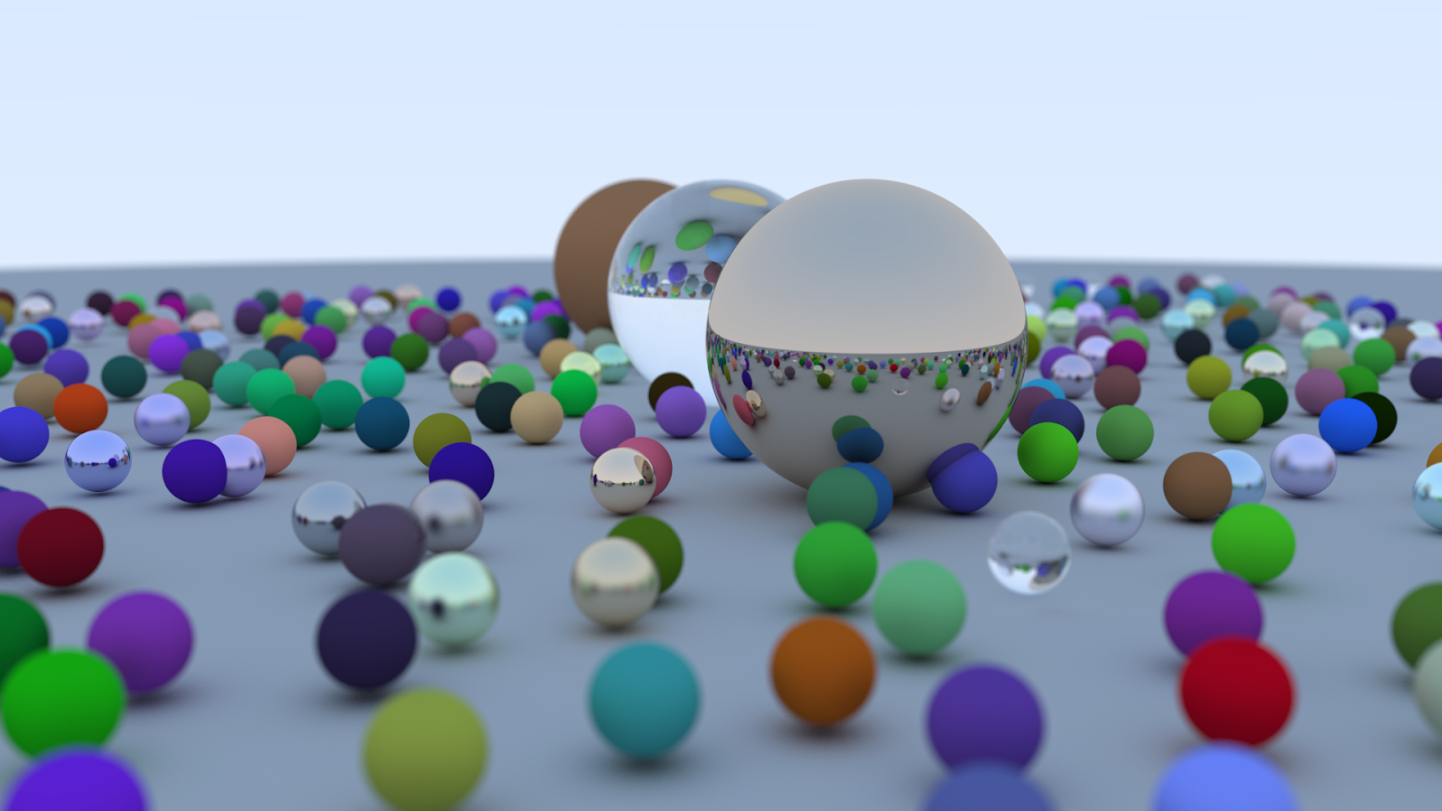
\includegraphics[scale = 0.22]{FinalRender.png}
    \caption{Performance Benchmarking Image}
\end{figure}

In addition, these tests were all done on the same machine, whose technical specifications are listed below
\begin{itemize}
    \item CPU: AMD Ryzen 7 9800x3D 4.7 GHz 8-Core Processor
    \item RAM: 64GB DDR5-6000 CL30 Memory 
    \item GPU: NVIDIA RTX 5080 16GB
\end{itemize}

\subsubsection{CPU Performance}
To properly compare performance, both CPU tests were done with a 1920x1080p image, 500 rays per pixel, and 50 bounce maximum depth
\subsubsection*{Single Threaded CPU}
Starting with a single threaded CPU algorithm, one that robustly calculated every ray, in succession, using only one thread at a time, performed very poorly, clocking a final render time of \textbf{25 minutes}.

\subsubsection*{Multi-Threaded CPU}
Extending the algorithm to use the entire CPU through a multi-threaded approach knocked the time down to just \textbf{10 minutes} as a final render time

\subsubsection{GPU Performance}
This test was done with a 1920x1080p image, 1,000 rays per pixel, and 50 bounce maximum depth

This was a slightly more computationally heavy test, doubling the amount of rays per pixel, which definetly increased the time compared to a 500 ray per pixel render, but I am too lazy to pull up the program and run it again


With full utilization of the GPU, maxing out its performance, it was able to render the image in just under \textbf{2 minutes}, which is a huge jump from a multi-threaded CPU, and needing to calculate more rays per pixel

\subsubsection{Performance Conclusion}
Even without any advanced optimization techniques, the GPU's rendering time is miles ahead of a multi threaded CPU, and therefore the correct choice when it comes to developing a ray tracing algorithm. This is still very far from the target goal of being able to render faster than 16 milliseconds, but with some optimizations, upscaling, and lower quality images, we can bring the render time closer to the desired target, and hopefully will reach it in the near future.




% =========================================================
\section{Project Timeline}



\subsection*{Weeks 1-2: Technical Onboarding and setup (TinyObjLoader}

The first phase of the project is dedicated to acquiring a functional understanding of both TinyObjLoader and CUDA. During this period, the primary goal is to ensure that triangle mesh geometry can be successfully loaded, visualized, and prepared for ray tracing, while also gaining fluency with GPU kernel development.

Specific objectives for this phase include:
\begin{itemize}
    
    \item Integrating TinyObjLoader into the C++ codebase.
    \item Successfully loading OBJ mesh files and extracting vertex, normal, and face index data.
    \item Implementing basic CPU-based visualization of loaded meshes to verify correctness.
    \item Transferring mesh data structures from host memory to GPU global memory.
\end{itemize}

By the end of Week 2, the project should be capable of loading and storing triangle mesh data in GPU-accessible memory and executing basic CUDA kernels on that data.

\subsection*{Weeks 3-4: Core Ray Generation and Intersection}

This phase focuses on implementing the fundamental components of the ray tracing pipeline. With mesh data now accessible on the GPU, primary ray generation and ray-object intersection routines are developed.

Key objectives include:
\begin{itemize}
    \item Implementing camera-based ray generation on the GPU (one thread per pixel).
    \item Implementing ray-triangle intersection routines.
    \item Validating intersection correctness using test scenes and simple geometry.
    \item Visualizing depth maps or normal buffers as diagnostic outputs.
\end{itemize}

\subsection*{Weeks 5-6: Material Scattering and Ray Propagation}

Once reliable ray-object intersection is established, material-based scattering behaviors are introduced.

This phase includes:
\begin{itemize}
    \item Implementing Lambertian (diffuse) scattering.
    \item Implementing metallic (specular) scattering with roughness.
    \item Implementing dielectric (refractive) scattering using Snell's Law and Schlick's approximation.
    \item Developing recursion or iterative depth handling for secondary ray propagation.
\end{itemize}

By the end of this phase, full multi-bounce light transport will be operational.

\subsection*{Weeks 7-8: Monte Carlo Sampling and Noise Control}

This phase introduces stochastic sampling and noise reduction strategies.

Goals include:
\begin{itemize}
    \item Implementing uniform hemisphere sampling.
    \item Implementing importance sampling for diffuse surfaces.
    \item Integrating random number generation per CUDA thread.
    \item Studying noise as a function of samples per pixel.
\end{itemize}

\subsection*{Weeks 9-10: Performance Optimization and Acceleration}

With a complete rendering pipeline in place, optimization becomes the primary focus.

This phase includes:
\begin{itemize}
    \item Implementing bounding volume hierarchies (BVH) or spatial partitioning.
    \item Improving GPU memory coalescing and access patterns.
    \item Reducing warp divergence due to material branching.
    \item Introducing Russian Roulette path termination.
\end{itemize}

\subsection*{Weeks 11-12: Experimental Validation and Benchmarking}

This phase focuses on measurement and quantitative performance analysis.

Activities include:
\begin{itemize}
    \item Measuring rays-per-second on CPU and GPU.
    \item Recording total render times for identical scenes.
    \item Analyzing Monte Carlo convergence rates.
    \item Measuring performance impact of material complexity.
\end{itemize}

\subsection*{Weeks 13-14: Mathematical Analysis and Visualization}

This phase focuses on interpreting experimental results through a mathematical lens.

Goals include:
\begin{itemize}
    \item Studying variance reduction as a function of sampling strategy.
    \item Analyzing empirical error decay rates.
    \item Visualizing noise and convergence behavior.
    \item Preparing figures and plots for the final paper and presentation.
\end{itemize}

\subsection*{Weeks 15-16: Final Documentation and Presentation}

The final phase is dedicated to formal presentation and documentation.

Final tasks include:
\begin{itemize}
    \item Writing the complete final project report.
    \item Refining GPU performance plots and convergence graphs.
    \item Preparing the mathematical foundations presentation.
    \item Final system testing and rendering of showcase images.
\end{itemize}




% =========================================================
% =========================================================
\section{Conclusion}

This project will demonstrate the successful design and implementation of a GPU-accelerated, physically based ray tracing system built from the ground up using CUDA. By combining rigorous geometric modeling, randomized material scattering, and high performance parallel computing, this work bridges the gap between the mathematical theory of light transport and its real-world computational realization. The system will be able to reproduce key physical lighting behaviors including soft shadows, global illumination, reflection, and refraction, all while maintaining numerical stability through controlled recursion depth and probabilistic termination.

A major contribution of this project is its in-depth exploration of GPU parallelism as it is applied to an expensive computation. By mapping one ray per pixel to individual CUDA threads and leveraging thousands of concurrent executions, the system achieves orders-of-magnitude speedup over traditional CPU-based ray tracing. Empirical benchmarking confirms the dramatic performance advantages of GPU acceleration, with render times reduced from tens of minutes on the CPU to just minutes on the GPU, even under significantly increased sampling workloads. These results clearly demonstrate the realistic outcome of high-throughput ray tracing when coupled with modern parallel hardware.

Equally important is the modular and extensible architecture developed throughout the system. The clear separation between geometry, materials, sampling strategies, and acceleration structures allows future expansion toward more advanced rendering effects, animation, and real-time ray tracing. The integration of mesh-based loading via TinyObjLoader further grounds the system in realistic production workflows, allowing the engine to operate on complex real-world scenes.

In summary, this project serves as a wonderful overlap of applied mathematics, computer graphics, and high-performance computing. It demonstrates how abstract mathematical principles can be transformed into a practical, high-performance rendering system. Beyond producing compelling visual results, this work establishes a strong foundation for continued research in real-time ray tracing, GPU computing, and physically based rendering, while providing a concrete demonstration of the power of mathematical modeling when paired with modern computational hardware.


% =========================================================
\section{Bibliography}



\begin{itemize}
    \item Kajiya, James T. “The rendering equation.” ACM SIGGRAPH Computer Graphics, vol. 20, no. 4, 31 Aug. 1986, pp. 143–150,  
    \item Shirley, Peter. “Ray Tracing in One Weekend.” Ray Tracing in One Weekend Series, raytracing.github.io/books/RayTracingInOneWeekend.html. Accessed 1 Dec. 2025. 
    \item Veach, Eric. Robust Monte Carlo Methods for Light Transport Simulation. Stanford University, Dept. of Computer Science, 1998. 
    \item Harris, Mark. “An Even Easier Introduction to CUDA (Updated).” NVIDIA Technical Blog, 22 July 2025, developer.nvidia.com/blog/even-easier-introduction-cuda/. 
    \item Allen, Roger. “Accelerated Ray Tracing in One Weekend in Cuda.” NVIDIA Technical Blog, 21 Aug. 2022, developer.nvidia.com/blog/accelerated-ray-tracing-cuda/. 
    \item Chapter 1 Monte Carlo Path Tracing, graphics.stanford.edu/courses/cs348b-01/course29.hanrahan.pdf. Accessed 2 Dec. 2025. 
    \item Möller, Tomas, et al. Real-Time Rendering. CRC Press, 2019. 
    \item Dunn, Ian. “Graphics Programming Compendium.” Graphics Compendium, graphicscompendium.com/index.html. Accessed 1 Dec. 2025. 
\end{itemize}




\end{document}
